\documentclass{beamer}
\usetheme{default}
\usepackage{mathtools}
\setbeamertemplate{footline}[frame number]

\title{[13] Interior-Point Method for Nuclear Norm Approximation with Application to System Identification}
\author{Author: Zhang Liu and Lieven Vandenberghe, 2009\\ \footnotesize Presentation by: Martin Hellkvist}

\newcommand{\mA}{\mathcal{A}}

\begin{document}
\begin{frame}[plain]
    \maketitle
\end{frame}
\begin{frame}{Summary}
	\begin{itemize}
		\item Nuclear Norm: $ ||X||_* =$ sum of singular values
		\item $ \min\,||X||_* $ typically has low rank solutions
		\begin{itemize}
			\item Can be cast as Semidefinite Program (SDP)
		\end{itemize}
		\item $ \min\,\text{rank}(X) $ is NP-hard
		\begin{itemize}
			\item System Identification
			\item Machine Learning
			\item Computer Vision
		\end{itemize}
		\item Contribution:
		\begin{itemize}
			\item Describe a more efficient interior-point method for high order problems with the structure that follows $ ||\cdot||_* $
		\end{itemize}
	\end{itemize}
\end{frame}

\begin{frame}{Nuclear Norm Approximation Problem}
	\begin{equation}
	\begin{split}
		&\text{minimize}~|| \mA (x) - B||_* \\
		&B \in \mathbb{R}^{p\times q}\\
		&\mA(x) = x_1A_1+x_2A_2+\dots+x_nA_n
	\end{split}
	\end{equation}
	is convex:
	\visible<2->{
		\begin{equation}
		\begin{split}
			&||\mA(\alpha x + (1 - \alpha)y) - B||_* = \\
			&||\alpha(\mA(x) - B)+(1-\alpha)(\mA(y)-B)||_* \leq\\
			&||\alpha(\mA(x) - B)||_*+||(1-\alpha)(\mA(y)-B)||_*=\\
			&\alpha||\mA(x) - B||_*+(1-\alpha)||\mA(y)-B||_*
		\end{split}
		\end{equation}
	}
\end{frame}
\begin{frame}{Nuclear Norm Approximation Problem}
	Can be cast as
	\begin{equation}
	\begin{split}
		&\text{minimize}~~~(\mathbf{tr}U + \mathbf{tr}V)/2\\
		&\text{subject to}~~\begin{bmatrix}
		U & (\mA(x)-B)^T\\
		\mA(x) - B & V
		\end{bmatrix} \succeq 0
	\end{split}
	\end{equation}
	Where $ U = U^T \in \mathbb{R}^{q\times q}$ and $ V=V^T \in \mathbb{R}^{p \times p} $ are new variables, and the problem is an SDP which is very difficult to solve for $ q \approx 100 $ and $ p\approx 100 $ for general purpose interior-point methods where $ \mathcal{O}(p^2q^2n) $
\end{frame}

\begin{frame}{Custom Interior-Point Method}
Exploiting the structure of 
	\begin{equation}
	\begin{split}
		&\text{minimize}~~~(\mathbf{tr}U + \mathbf{tr}V)/2\\
		&\text{subject to}~~\begin{bmatrix}
		U & (\mA(x)-B)^T\\
		\mA(x) - B & V
		\end{bmatrix} \succeq 0
	\end{split}
	\end{equation}
We need to solve the following linear equation system
	\begin{equation}
	\mA_{\text{adj}}(\Delta Z) = r, ~~ \begin{bmatrix}
	\Delta U & \mA(\Delta x)^T\\
	\mA(\Delta x) & \Delta V
	\end{bmatrix}+ T \begin{bmatrix}
	0 & \Delta Z^T\\
	\Delta Z & 0
	\end{bmatrix}T = R
	\end{equation}
	which can be solved by first finding $ \Delta x $
	\begin{equation}
		\tilde{\mA}_\text{adj}(\mathcal{S}^{-1}(\tilde{\mA}(\Delta x)))=\tilde{\mA}_\text{adj}(\mathcal{S}^{-1}(\tilde{R}_{21})) -r
	\end{equation}
	which gives $ \Delta Z $ and in turn $ \Delta U $ and $ \Delta V $
\end{frame}

\begin{frame}{Key step}
Solving for $ \Delta x $ looks complicated
	\begin{equation}
		\tilde{\mA}_\text{adj}(\mathcal{S}^{-1}(\tilde{\mA}(\Delta x)))=\tilde{\mA}_\text{adj}(\mathcal{S}^{-1}(\tilde{R}_{21})) -r
	\end{equation}
However ,
\begin{equation}
	\mathcal{S}(X) = \mathcal{L}(\mathcal{L}_\text{adj}(X))
\end{equation}
\visible<2->{
	where the inverses is ``simply'' defined as:
	\begin{equation}
		\mathcal{L}^{-1}(X)_{ij} = 
		\left\{\begin{matrix*}[l]
			(X_{ij} - \sigma_i\sigma_jX_{ji})/\sqrt{1-\sigma_i^2\sigma_j^2},\, &i<j\\
			X_{ii}/\sqrt{1+\sigma_i^2},\,&i=j\\
			X_{ij},\,&i>j
		\end{matrix*}\right.
	\end{equation}
	and its adjoint $ \mathcal{L}_\text{adj}^{-1} $ in a similar fashion
}
\end{frame}
\begin{frame}{Complexity reduction}
	\begin{itemize}
		\item From $ \mathcal{O}(p^2q^2n) $ to $ \mathcal{O}(pqn^2) $
		\item Works for large problems
	\end{itemize}
	 \begin{figure}[h]
		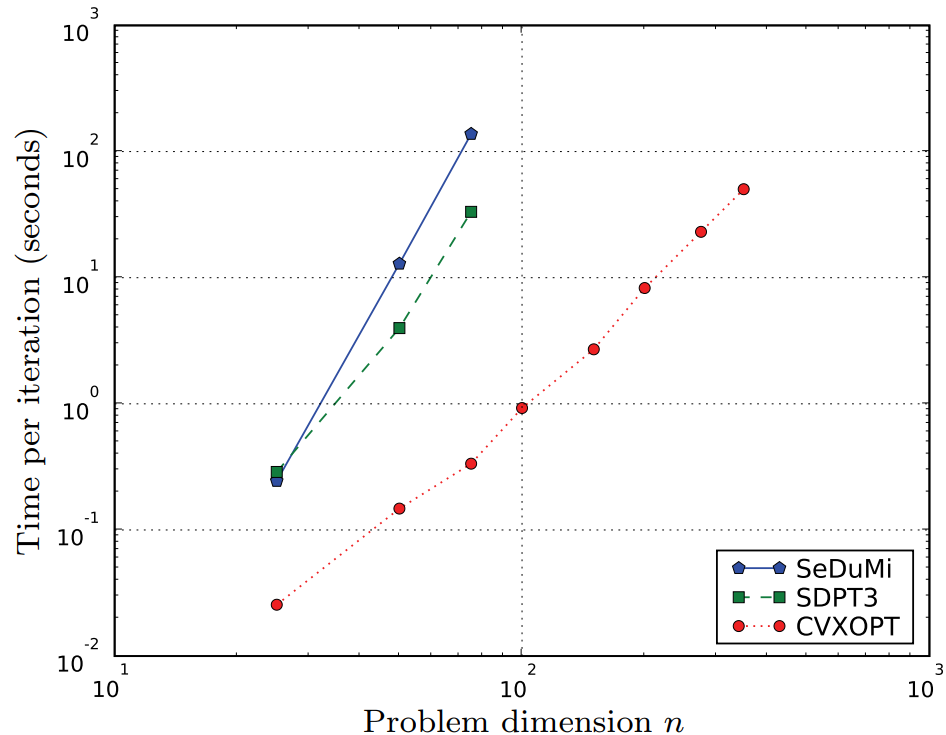
\includegraphics[width=0.55\linewidth]{Fig_1}
		\caption{Solving randomly generated problems for $p=q=n $}
		\label{}
	\end{figure}
\end{frame}

\begin{frame}{Subspace Identification}
	Given inputs $ u(t) $ and output measurements $ y_\text{meas}(t) $ we can find low rank state space representation by
	\begin{equation}
	\min ||YU^\perp||_* + \gamma \sum_{t=0}^N ||y(t)-y_\text{meas}(t)||_2^2
	\end{equation}
	\visible<2->{
		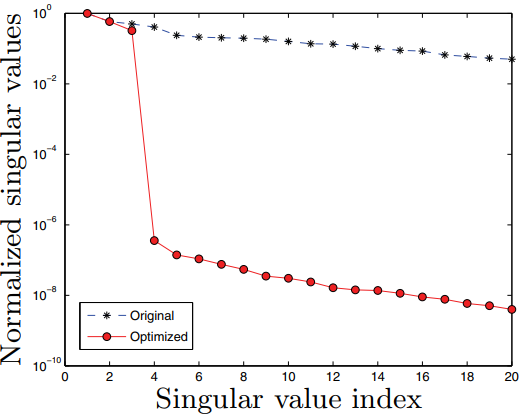
\includegraphics[width=.45\linewidth]{Fig_4}
	}
	\visible<3->{
		\hfill
		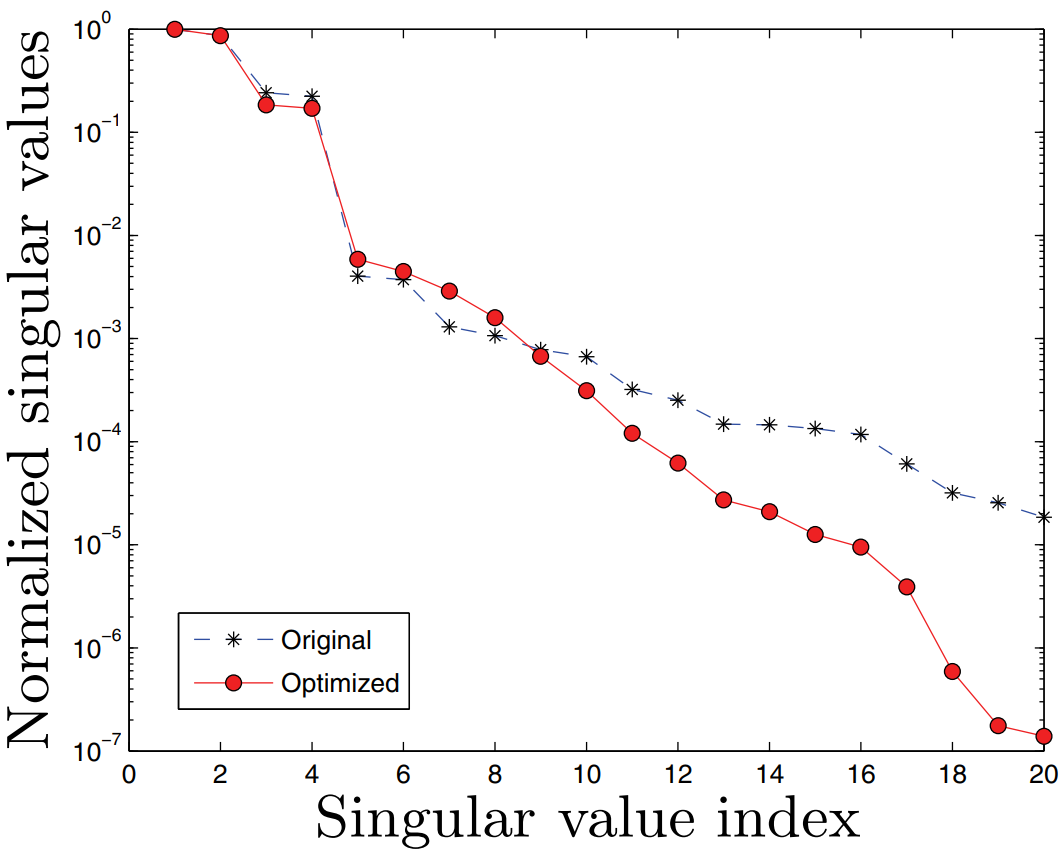
\includegraphics[width=.45\linewidth]{Fig_6b}
	}
\end{frame}
\begin{frame}{Shortcomings and Extensions}
Shortcomings
	\begin{itemize}
		\item Lackluster comments on numerical results
		\item Unclear what is ``the trick''
	\end{itemize}
Extensions
	\begin{itemize}
		\item How does quadratic terms affect the equations?
		\item Least Norm Problem (adds $ \mathcal{F}(X)=g $ to SDP constraints)
	\end{itemize}
\end{frame}
\end{document}
